\documentclass{article}
\usepackage[nonatbib]{project}
\usepackage{watml}

\usepackage[normalem]{ulem}
\usepackage{setspace}
% use Times
\usepackage{times}
% For figures
\usepackage{graphicx} % more modern
%\usepackage{epsfig} % less modern
%\usepackage{subfig} 

% path to figure folder
\graphicspath{{../fig/}}

% bib file for references
\addbibresource{project.bib}


\title{Replace with your title}

\author{
	Yao-Liang Yu \\
	School of Computer Science\\
	University of Waterloo\\
	Waterloo, ON, N2L 3G1 \\
	\texttt{yaoliang.yu@uwaterloo.ca} \\
	{\color{red} report due: August 15}
}

\begin{document}
\maketitle

\begin{abstract}
	Put here a brief summary of the project: what is it about and what are the main results. You also need to submit your code for reproducibility (a github \href{https://github.com/}{link} suffices). Be concise and to the point. Please limit the report to less than ($\leq$) \textbf{4 pages} (references excluded).
\end{abstract}

\section{Introduction}
In this section you are going to present a brief background and motivation of your project. Consider summarizing the entire report in one overarching figure, such as \Cref{fig:eqv_sde_traj}.

\begin{figure*}[h]
	\centering
	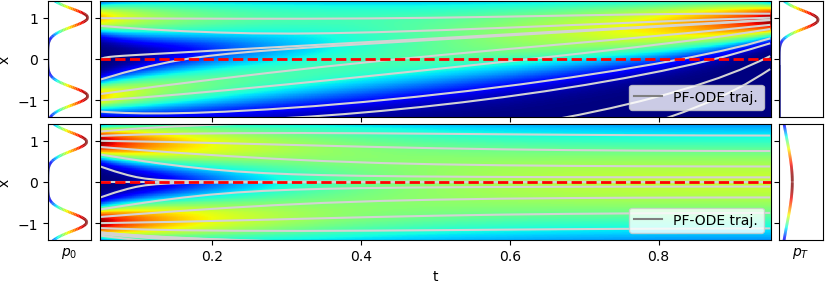
\includegraphics[width=0.9 \textwidth]{traj_combined.png} ~~~
	\raisebox{0.18\height}{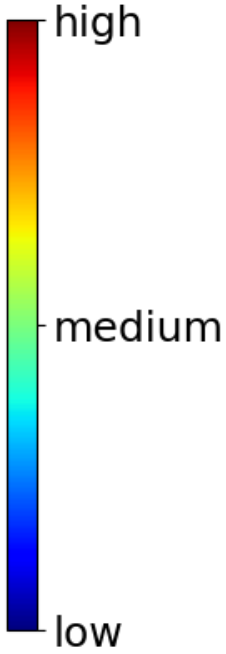
\includegraphics[width=0.07 \textwidth]{cbar3.png}}
	\caption{The evolution of $p_t$ driven by diffusion processes where the data distribution $p_0$ is invariant under flipping with respect to the origin. We also plot the PF-ODE trajectories to visualize the transition direction of $p_t(x)$. The upper plot has $f(x, t) = \frac{1-x}{1-t}$ and $g(t) = 1$. The lower is VP-SDE with $\alpha_t = 1 -t$. For both processes, $T = 0.95$.}
	\label{fig:eqv_sde_traj}
\end{figure*}

\section{Related Works}
Perform a reasonably thorough review of relevant literature. Has your approach, or one of similar nature, been considered before? By whom? What are the differences or limitations (if any)?

\section{Main Results}
Formulate your problem precisely (mathematically) and present the main methodology. Explain and justify each of your design choices, with some ablation studies to back them up.

\begin{table}[t]
	\centering
	\caption{Model Comparison on 28x28x1 Rotated MNIST (Group C4).
		\footnotesize{*} indicates author-reported values.
	}
	\setlength\tabcolsep{12pt}
	\begin{tabular}{@{}lcccccc@{}}
		\toprule
		\multirow{2}{*}{Model} & \multicolumn{4}{c}{FID$\downarrow$} & \multicolumn{1}{c}{Inv-FID$\downarrow$} & \multicolumn{1}{c}{$\Delta\hat x_0\downarrow$}                                                   \\  \cmidrule{2-7}
		                       & $1\%$                               & $5\%$                                   & $10\%$                                         & $100\%$               & $100\%$       & $100\%$ \\ \midrule
		SPDiff                 & 5.97                                & \textbf{3.05}                           & 3.47                                           & 2.81                  & 2.21          & 0.2997  \\
		SPDiff+WT              & 5.80                                & 3.34                                    & 3.57                                           & 3.50                  & 2.20          & 0.0004  \\
		SPDiff+OC              & 6.10                                & 3.09                                    & 3.45                                           & 2.82                  & 2.12          & 0.0002  \\
		SPDiff+Reg             & \textbf{5.42}                       & 3.69                                    & \textbf{2.83}                                  & 2.75                  & 2.09          & 0.1806  \\
		SPDiff+Reg+OC          & 5.64                                & 3.67                                    & 2.86                                           & \textbf{2.64}         & \textbf{2.07} & 0.0002  \\
		SP-GAN                 & 149\textsuperscript{*}              & 99\textsuperscript{*}                   & 88\textsuperscript{*}                          & 81\textsuperscript{*} & --            & --      \\
		SP-GAN (Reprod.)       & 16.59                               & 11.28                                   & 9.02                                           & 10.95                 & 19.92         & --      \\ \bottomrule
	\end{tabular}
	\label{tab:fid-rot-mnist}
\end{table}

Please always give proper citations to prior work or results. Be precise and concise. Pay some attention to the organization and layout of the entire paper. Add variety (table, curves, bar graph, scatter plot, violin plot, pseudocode, \etc) and report statistical deviation (over at least 3$\sim$5 runs).

\begin{algorithm}[H]
	\DontPrintSemicolon
	\KwIn{$\wv_0 \in \dom f$}
	\For{$k = 0, 1, 2, \ldots$}{

		$\gv_{k} \gets \tfrac1n\sum_{i=1}^n \nabla \ell_i(\wv_k)$ \tcp*{compute full gradient at epoch $k$}

		$\wv_{k, 0} \gets \wv_k$

		\For{$t=0,\ldots, m-1$}{

			randomly draw $i_t = i$ with probability $p_i$

			$\gv_{k,t} \gets \red{\gv_{k}} - \tfrac{1}{\orange{n p_{i_t}}}\nabla \ell_{i_t}(\wv_k) + \tfrac{1}{\orange{n p_{i_t}}} \nabla \ell_{i_t}(\wv_{k,t})$ \tcp*{amortized gradient}

			$\wv_{k, t+1} \gets \prox[\eta_k]{r}(\wv_{k, t} - \eta_k \gv_{k,t})$ \tcp*{stochastic proximal gradient}
		}

		$\wv_{k+1} \gets \tfrac1m\sum_{t=1}^m \wv_{k, t}$ \tcp*{in practice, can also do $\wv_{k+1} \gets \wv_{k, m}$}
	}
	\caption{Stochastic variance reduced proximal gradient}
\end{algorithm}


\section{Conclusion}
What have we learned? What limitations or directions do you think are worth exploring in the future?


\newpage

\section*{Acknowledgement}
Thank people who have helped or influenced you in this project. \Cref{fig:eqv_sde_traj} and \Cref{tab:fid-rot-mnist} are from \citet{LuSY24}.

\nocite{*}
\printbibliography[title=References]


\end{document}